\documentclass{article}

%
%   Packages
%
\usepackage[a4paper,top=2cm,bottom=2cm,left=2cm,right=2cm, inner=3cm]{geometry}
\usepackage{graphicx}
\usepackage{biblatex}
\usepackage[acronym]{glossaries}
\usepackage[italian]{babel}
\usepackage{csquotes}

%
%   Utilities and costants
%
\def\blankpage{
    \clearpage
    \thispagestyle{empty}
    \addtocounter{page}{-1}
    \null
    \clearpage
}
    

%
%   Acronyms
%
\newacronym{ms}{MS}{\textit{Mobile system}}
\newacronym{dos}{DOS}{\textit{Denial Of Service}}
\newacronym{iot}{IOT}{\textit{Internet Of Things}}
\newacronym{ran}{RAN}{\textit{Radio Access Network}}
\newacronym{ue}{UE}{\textit{User Equipment}}
\newacronym{bs}{BS}{\textit{Base Station}}
\newacronym{sim}{SIM}{\textit{Subscriber Identity Module}}
\newacronym{mtso}{MTSO}{\textit{Mobile Telephone Switching Office}}
\newacronym{fdma}{FDMA}{\textit{Frequency Division Multiple access}}
\newacronym{gsm}{GSM}{\textit{Global System for Mobile Communication}}
\newacronym{sms}{SMS}{\textit{Short Message Service}}
\newacronym{bss}{BSS}{\textit{Base Station Subsystem}}
\newacronym{nss}{NSS}{\textit{Network Switching Subsystem}}
\newacronym{msc}{MSC}{\textit{Mobile  Switching  Centre}}
\newacronym{ptsn}{PTSN}{\textit{Public switched telephone network}}
\newacronym{hlr}{HLR}{\textit{Home Location Register}}
\newacronym{vlr}{VLR}{\textit{Visitor Location Register}}
\newacronym{eir}{EIR}{\textit{Equipment Identity Register}}
\newacronym{auc}{AuC}{\textit{Authentication Center}}
\newacronym{gprs}{GPRS}{\textit{General Packet Radio Service}}
\newacronym{sgsn}{SGSN}{\textit{Serving GPRS Support Node}}
\newacronym{wcdma}{W-CDMA}{\textit{Wideband Code Division Multiple Access}}
\newacronym{umts}{UMTS}{\textit{Universal Mobile Telecommunications System}}
\newacronym{ggsn}{GGSN}{\textit{Gateway GPRS Support Node}}
\newacronym{ip}{IP}{\textit{Internet Protocol}}
\newacronym{hss}{HSS}{\textit{Home Subscriber Server}}
\newacronym{mme}{MME}{\textit{Mobility Management Entity}}
\newacronym{sgw}{S-GW}{\textit{Serving - Gateway}}
\newacronym{lte}{LTE}{\textit{Long Term Evolution Standard}}
\newacronym{pgw}{P-GW}{\textit{Packet data network - Gateway}}
\newacronym{pcrf}{PCRF}{\textit{Policy Control and Charging Rules Function}}
\newacronym{sba}{SBA}{\textit{Service Base Architecture}}
\newacronym{sdn}{SDN}{\textit{Software Defined Network}}
\newacronym{ddos}{DDOS}{\textit{Distributed Denial Of Service}}
\newacronym{aka}{AKA}{\textit{Authentication and Key Agreement}}
\newacronym{imsi}{IMSI}{\textit{International Mobile Subscriber Identity}}
\newacronym{imei}{IMEI}{\textit{International Mobile Equipment Identity}}
\newacronym{tmsi}{TMSI}{\textit{Temporary MobileSubscriber Identity}}
\newacronym{sres}{SRES}{\textit{Signed Response}}
\newacronym{suci}{SUCI}{\textit{Subscription Concealed Identifier}}
\newacronym{ik}{IK}{\textit{Integrity Key}}
\newacronym{snn}{SNN}{\textit{Serving Network Name}}
\newacronym{tps}{TPS}{\textit{Transation Per Second}}
\newacronym{nfv}{NFV}{\textit{Network Function Virtualization}}
\newacronym{mitm}{MITM}{\textit{Man In The Middle}}
\newacronym{ecies}{ECIES}{\textit{Elliptic Curve Integrated Encryption Scheme}}
\newacronym{supi}{SUPI}{\textit{Subscription Permanent Identifier}}

\makenoidxglossaries

%
%   References
%
\addbibresource{formats/references.bib}

%
%   Document
%
\begin{document}
    \begin{titlepage}
  \begin{center}
    
\includegraphics[width=0.3\textwidth]{images/unipd.png}
    \hfill
    
\includegraphics[width=0.3\textwidth]{images/dei.png}
  \end{center}
  \begin{center}
    \vspace{3cm}
    \large
    \MakeUppercase{
      \textbf{
        Dipartimento di ingegneria dell'informazione\\
        \vspace{0.5cm}
        Corso di laurea in Ingegneria Informatica\\
      }
    }
    \vspace{5cm}
    \MakeUppercase{
      \textbf{
        Attacco di tipo Denial of Service alle reti cellulari\\
      }
    }
    \vspace{5cm}
    \begin{flushleft}
      \textbf{
        Relatore: Prof. Mauro Migliardi\\
      }
    \end{flushleft}
    \vspace{1cm}
    \begin{flushright}
      \textbf{
        Laureando: Stefano Leggio\\
      }
    \end{flushright}
    \vspace{2cm}
    \MakeUppercase{
      \textbf{
        Anno accademico: 2020-2021\\
      }
    }
    \vspace{0.5cm}
    \textbf{
      Data di laurea:
    }
  \end{center}
\end{titlepage}
    \blankpage
    \tableofcontents{}
    \clearpage
    \listoffigures
    \clearpage
    \printnoidxglossary[type=acronym, title={Elenco delle abbreviazioni}]
    \printacronyms
    \clearpage
    \section{Introduzione}
Le reti cellulari rappresentano un punto nevralgico per le nostre comunicazioni.
Per questo, la loro sicurezza è fondamentale per garantire un normale Funzionamento
di tutti i servizi a cui ormai abituati.
In questa tesi si tratterà della loro struttura e funzionamento, analizzando le diverse
tecnologie cellulari che con il tempo si sono susseguite. Dopodichè si procederà ad analizzare
nel dettaglio i meccanismi di autenticazione dei dispositivi, mettendo in luce le rispettive vulnerabilità
per le diverse tecnologie cellulari. Sfruttando delle vulnerabilità nel sistema di autenticazione si dimostrerà
come un attacco di tipo Denial of Service sia possibile, spiegando le possibili disastrose conseguenze che 
potrebbe comportare.
    \clearpage
    \chapter{La rete cellulare}
La rete cellulare è la struttura \textit{hardware} e \textit{software} che consente il corretto
funzionamento delle comunicazioni tramite i dispositivi cellulari, dalle normali comunicazioni vocali alle \textit{smart cities} nel 5G.\\
Grazie ad una fitta rete di antenne, i gestori telefonici riescono a garantire il servizio per la  gran parte del territorio mondiale.
\begin{figure}[h]
    \centering
    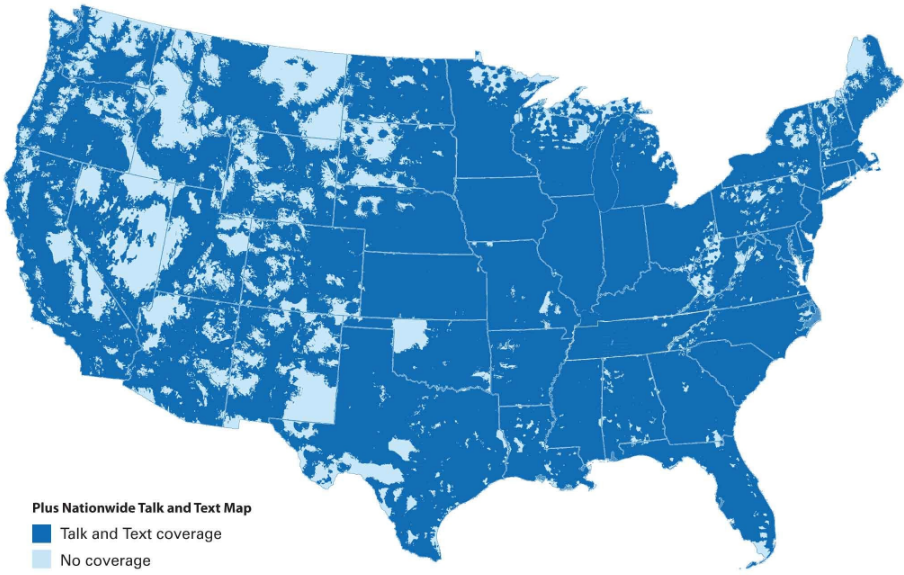
\includegraphics[width=0.7\textwidth]{images/att-coverage.png}
    \caption{Mappa compertura AT\&T negli USA}
\end{figure}\\

\clearpage

\section{Struttura}
La loro struttura e architectura hanno subito numerosi cambiamenti nel corso delle generazioni, in particolare con la rete
5G.\\
Si possono comunque identificare degli elementi chiave che sono presenti in tutte le generazioni:
\begin{itemize}
    \item MS \textit{Mobile System} ovvero il dispositivo cellulare, in alcune generazioni questo acronimo è leggermente diverso, come per esempio dal 3G è
    lo \textit{User Equipment} (UE).
    \item RAN \textit{Radio access network} ovvero l'infrastruttura fisica di antenne per la ricezione e trasmissione di informazioni per il dispositivo
    \item \textit{Core network} ovvero i componenti della sua architettura
\end{itemize}
\begin{figure}[h]
    \centering
    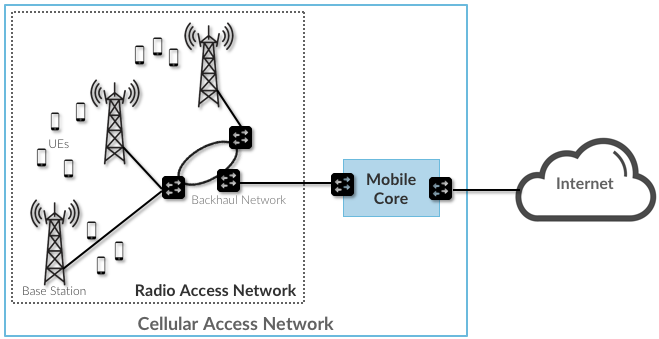
\includegraphics[width=0.7\textwidth]{images/cellular-network-basic-scheme.png}
    \caption{Schema di una rete cellulare}
\end{figure}
La RAN è composta ripetitori di segnale chiamati \textit{base station}. 
Questi vengono disposti in modo capillare sul territorio, suddividendolo in diverse aree di competenza chiamate celle. Ognuna di queste può gestire
un numero limitato di dispositivi in contemporanea, per questo, in caso di aree densamente popolate vengono 
ridotte le aree di competenza di ciascuna antenna. Le celle quindi, possono avere una dimensione variabile che dipende dal contesto in cui devono essere inserite.
\begin{figure}[h]
    \centering
    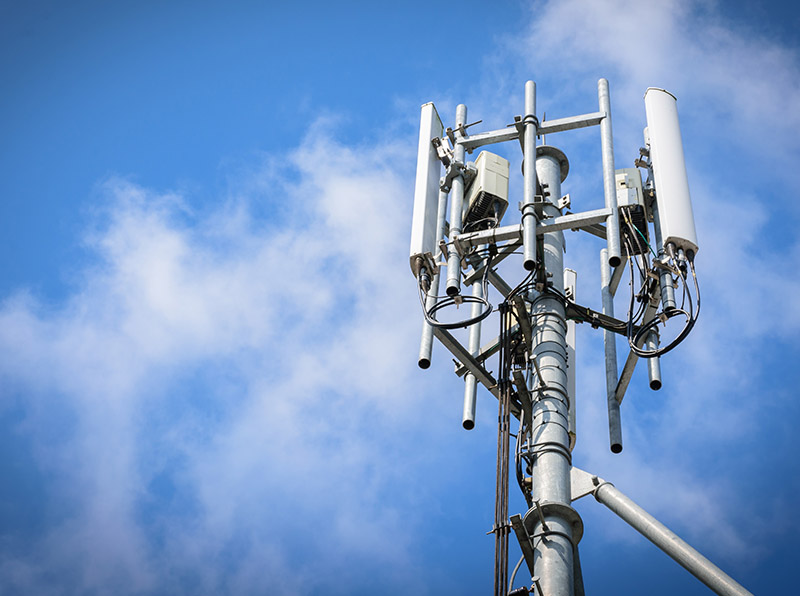
\includegraphics[width=0.5\textwidth]{images/base-station.jpg}
    \caption{Base station}
\end{figure}\\
Ogni cella ha un determinato raggio di azione che dipende dalle caratteristiche fisiche dell'antenna stessa. Inoltre, 
ha a disposizione un determinato range di frequenze su cui instaurare la comunicazione con i vari dispositivi, che solitamente
sono differenti rispetto a quelle usate dalle celle vicine per evitare interferenze.
Celle sufficientemente distanti possono utilizzare le stesse frequenze poiché non corrono il rischio di interferenza, questo rappresenta
un grande vantaggio per questa tecnologia.\\
\clearpage
\noindent Per identificare e autenticare ogni MS nella rete è necessario che sia fornito del \textit{Subscriber Identity Module} (SIM), ossia una scheda fisica 
che contiene le chiavi per autenticarsi alla rete.
\begin{figure}[h]
    \centering
    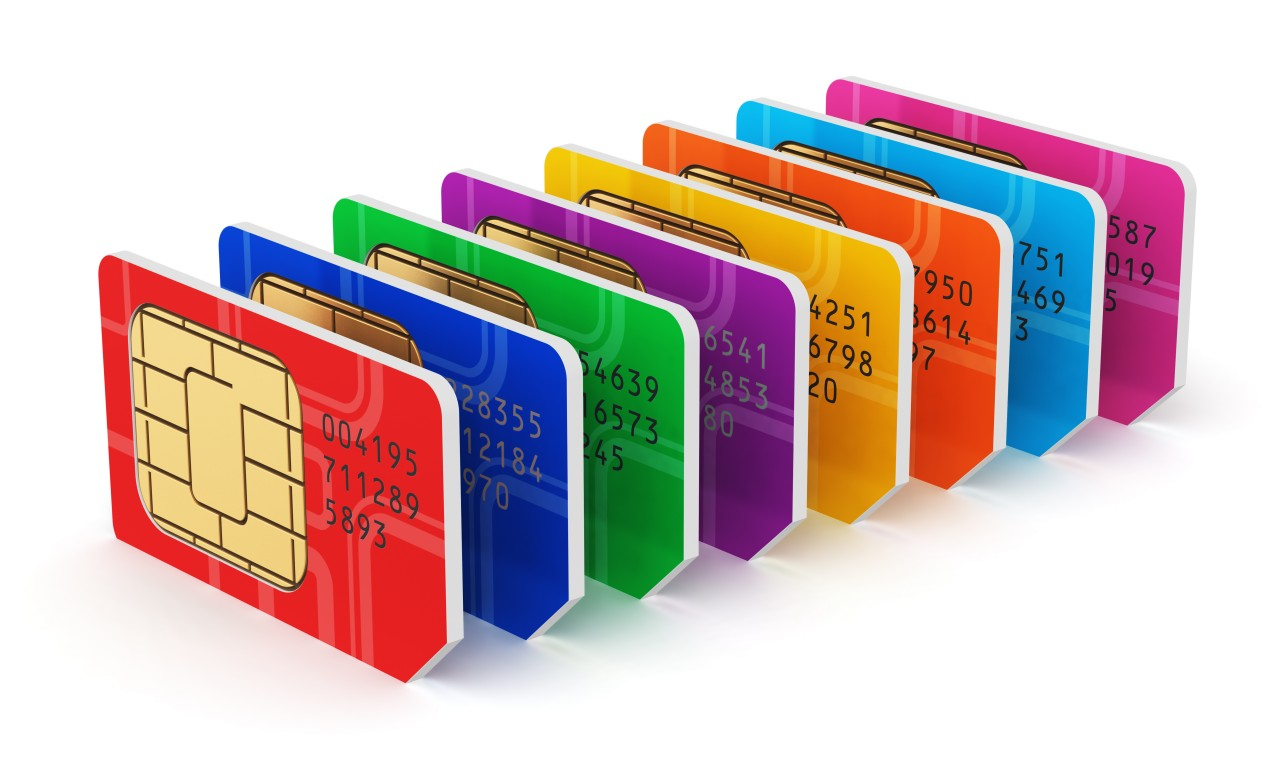
\includegraphics[width=0.5\textwidth]{images/simcard.jpg}
    \caption{\textit{Subscriber Identity Module}}
\end{figure}

\section{Architettura}
L'architettura di una rete cellulare è l'insieme dei componenti che permettono il suo corretto funzionamento come l'autenticazione e lo smistamento delle informazioni.\\
Nella sezione seguente verranno trattate nel dettaglio tutte le architetture: dal 1G al 5G, elencando i loro componenti principali. Si può comunque stilare una lista di elementi 
che devono essere in una architettura cellulare:
\begin{itemize}
    \item Archivio delle chiavi di autenticazione dei \textit{subscribers}.
    \item Archivio della posizione dei \textit{subscribers}, per permettere il raggiungimento del MS.
    \item Un \textit{controller} centrale che si occupa di interpellare gli archivi e smistare le informazioni.
    \item Componente per la commutazione a pacchetto, in caso la rete si interfacci a \textit{internet}.
\end{itemize}
    \clearpage
    \chapter{Generazioni cellulari}
Nel corso degli anni, si sono susseguite diverse generazioni di tecnologie cellulari, che hanno apportato
notevoli cambiamenti alla loro architettura e infrastruttura per consentire il raggiungimento di prestazioni migliori\cite{architecture-evolution}.\\
Di seguito verranno presentati le principali caratteristiche
delle diverse generazioni cellulari, in modo tale da rendere di facile comprensione l'analisi dei meccanismi
di autenticazione che verranno approfonditi nelle prossime sezioni.\\
Oltre ad elencare le principali caratteristiche di ogni generazione verranno analizzate nel dettaglio le specifiche  
dell'architettura di rete.
\begin{figure}[ht]
    \centering
    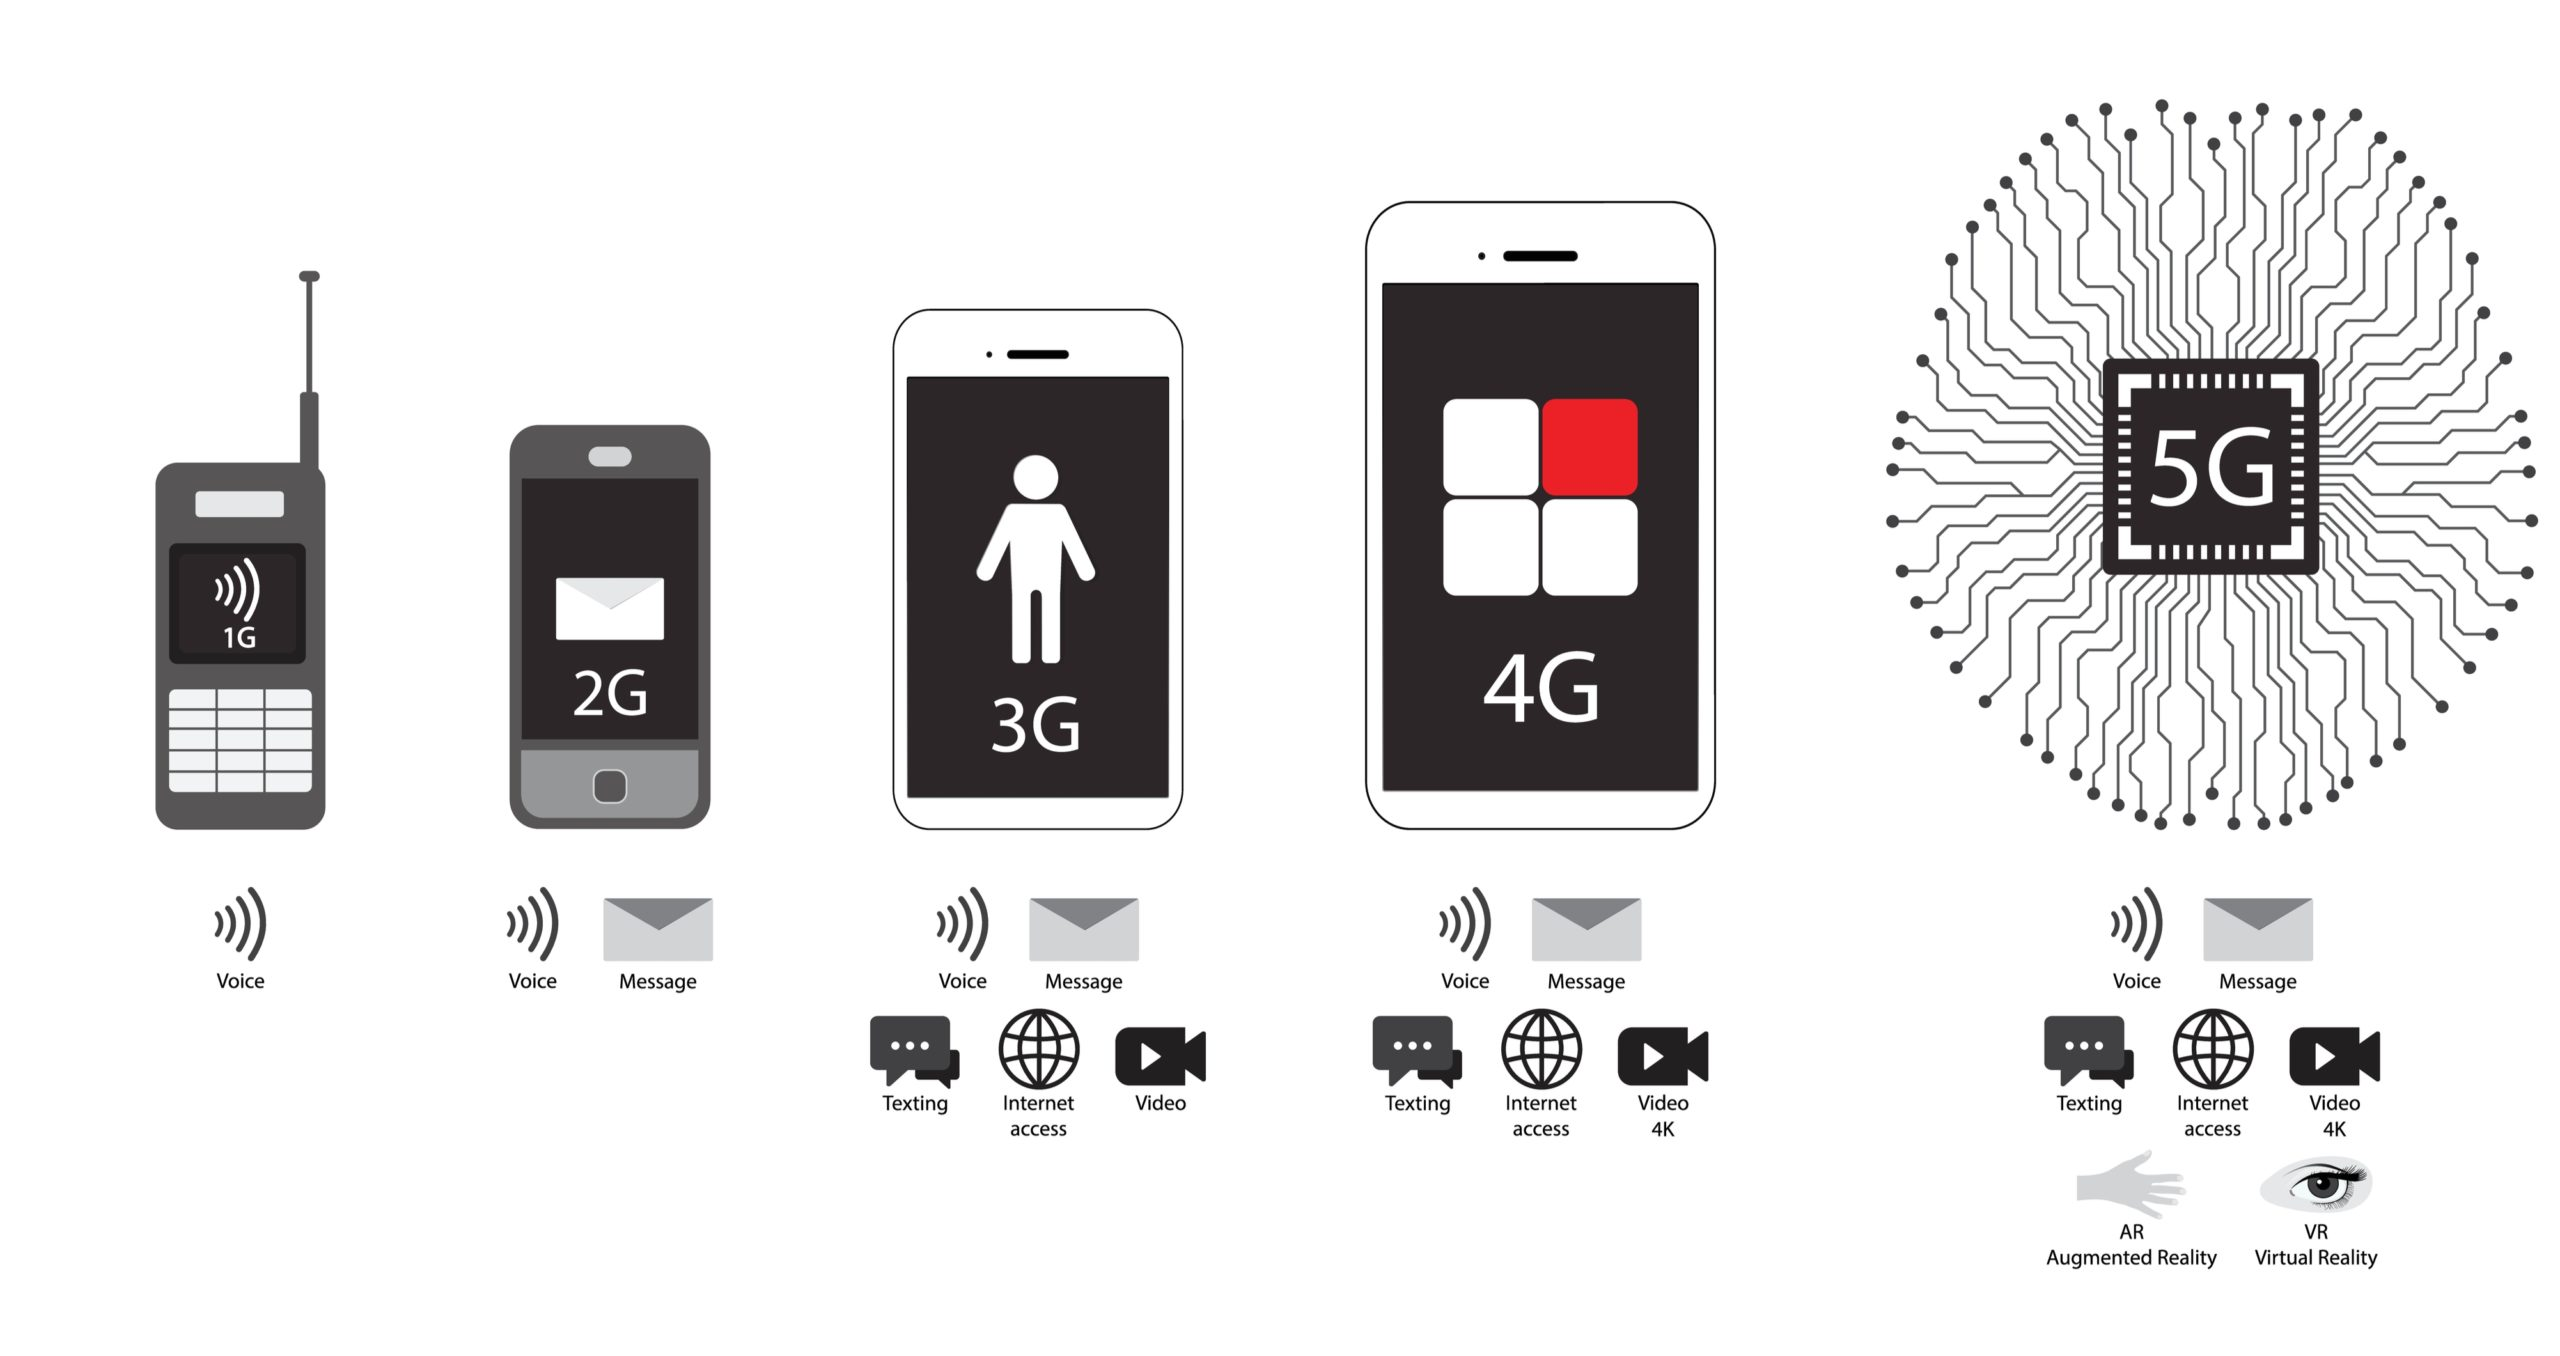
\includegraphics[width=0.7\textwidth]{images/generations-scheme.jpg}
    \caption{Schema delle generazioni cellulari}
\end{figure}

\clearpage

\section{1G}
La generazione 1G è uno dei primi standard di comunicazione cellulare. Il suo funzionamento era completamente analogico 
e ormai è stata rimpiazzata totalmente dalle generazioni digitali successive.\\
L'architettura di questa generazione è molto semplice, è composta da tre componenti principali:
\begin{itemize}
    \item Antenne per la trasmissione
    \item \textit{Mobile Telephone Switching Office} (MTSO)
    \item Unità mobile (cellulare)
\end{itemize}
\begin{figure}[ht]
    \centering
    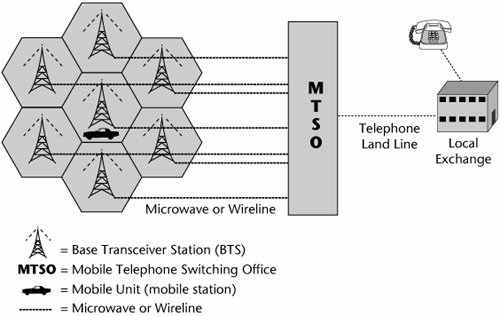
\includegraphics[width=0.7\textwidth]{images/1g.jpg}
    \caption{Architettura 1G}
\end{figure}
Si basava sulla \textit{frequency-division multiple access} (FDMA) in cui ogni dispositivo che si connetteva alla stazione radio
aveva assegnata una specifica sotto banda\cite{generations}.

\clearpage

\section{2G}
A differenza della prima generazione, la seconda introuduce per la prima volta una rete completamente digitale.
Questa tecnologia cellulare è composta da diverse versioni che si sono susseguite nel corso degli anni aggiungendo nuove 
funzionalità.
Anche la sua architettura subisce delle modifiche, per questo verranno trattate separatamente in seguito.
\subsubsection{GSM}
Il GSM, ovvero \textit{Global System for Mobile Communications}\cite{gsm} è uno standard di seconda generazione che introuduce importanti novità.\\
Le principali caratteristiche introdotte sono:
\begin{itemize}
    \item Maggiori velocità di trasmissione
    \item Cifratura della comunicazione
    \item Introduzione di nuovi servizi come gli SMS
\end{itemize}
\begin{figure}[ht]
    \centering
    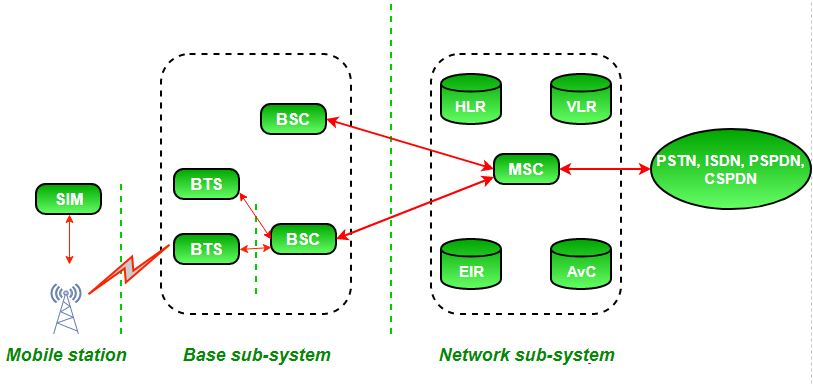
\includegraphics[width=0.7\textwidth]{images/2g-gsm.jpg}
    \caption{Architettura GSM}
\end{figure}
La sua architettura è composta da due macro aree: La BSS \textit{Base Station SubSystem} e la NSS \textit{Network SubSystem}.
Il BSS è l'insieme delle antenne ricevitori che rappresentano il primo collegamento con il MS, mentre il NSS rappresenta il \textit{core network} del GSM.\\
Il NSS è formato dai seguenti componenti:
\begin{itemize}
    \item \textit{Mobile Switching Centre} (MSC) è l'elemento centrale dell'atchitettura GSM, si occupa di interfacciare i BTS con la rete telefonica PTSN.
    \item \textit{Home Location Register} (HLR) \textit{database} centrale che contiene informazioni inerenti a tutti i \textit{subscribers}, molte delle informazioni
    che contiene sono dei puntatori agli archivi seguenti.
    \item \textit{Visitor Location Register} (VLR) \textit{database} che memorizza la posizione degli utenti.
    \item \textit{Equipment Identity Register} (EIR) \textit{database} di identificazione degli IMEI dei dispositivi. Grazie a questo archivio è possibile creare delle \textit{blacklist}
    per evitare l'accesso a determinati dispositivi.
    con l'autenticazione.
    \item \textit{Authenticaton Center} (AuC) \textit{database} di informazioni di sicurezza associate agli utenti registrati.
\end{itemize}

\clearpage

\subsection{GPRS}
La rete \textit{General Packet Radio Service} (GPRS)\cite{gprs-edge} introduce per la prima volta un trasferimento dati a commutazione di pacchetto per rendere 
possibile l'utilizzo dei servizi \textit{internet} con il proprio dispositivo cellulare\cite{gsm-architecture}.
La sua architettura è la stessa di quella del GSM ma con dei componenti aggiuntivi che consentono la trasmissione dei pacchetti. 
Per esempio, il \textit{Serving GPRS Support Node} (SGSN) è un componente per la gestione dei dispositivi connessi alla rete.
\begin{figure}[ht]
    \centering
    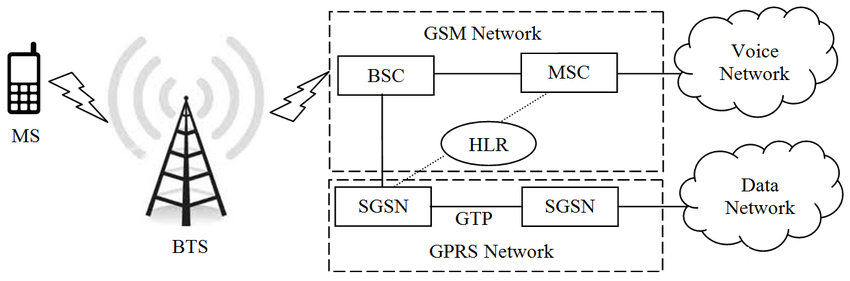
\includegraphics[width=0.7\textwidth]{images/2g-gprs.png}
    \caption{Architettura GPRS}
\end{figure}
\subsection{EDGE}
Evoluzione del GPRS che consente maggiori velocità, l'architettura resta invariata\cite{gprs-edge}.

\clearpage

\section{3G}
L'architettura della terza generazione riprende quella già vista nella seconda. Infatti, questa generazione ha avuto come principale obbiettivo 
quello di consolidare l'integrazione della rete internet nei sistemi cellulari ed aumentare la velocità di trasmissione per consentire l'utilizzo 
di nuovi servizi.\\
L'accesso al canale radio avviene con la tecnologia \textit{Wideband Code Division Multiple Access} (W-DCMA) con canale di banda 5 MHz.

\subsection{UMTS}
L'UMTS ovvero \textit{Universal Mobile Telecommunications System}\cite{umts} è il primo standard di terza generazione.
La sua architettura è composta dai seguenti elementi principali:
\begin{itemize}
    \item \textit{Mobile Switching Centre}, componente che ha la stessa funzione di quello in 2G, questa volta il VLR è integrato al suo interno.
    \item HLR/AuC e EIR
    \item SGSN e GGSN componenti ripresi dalla rete GPRS per la commutazione a pacchetto.
\end{itemize}
\begin{figure}[ht]
    \centering
    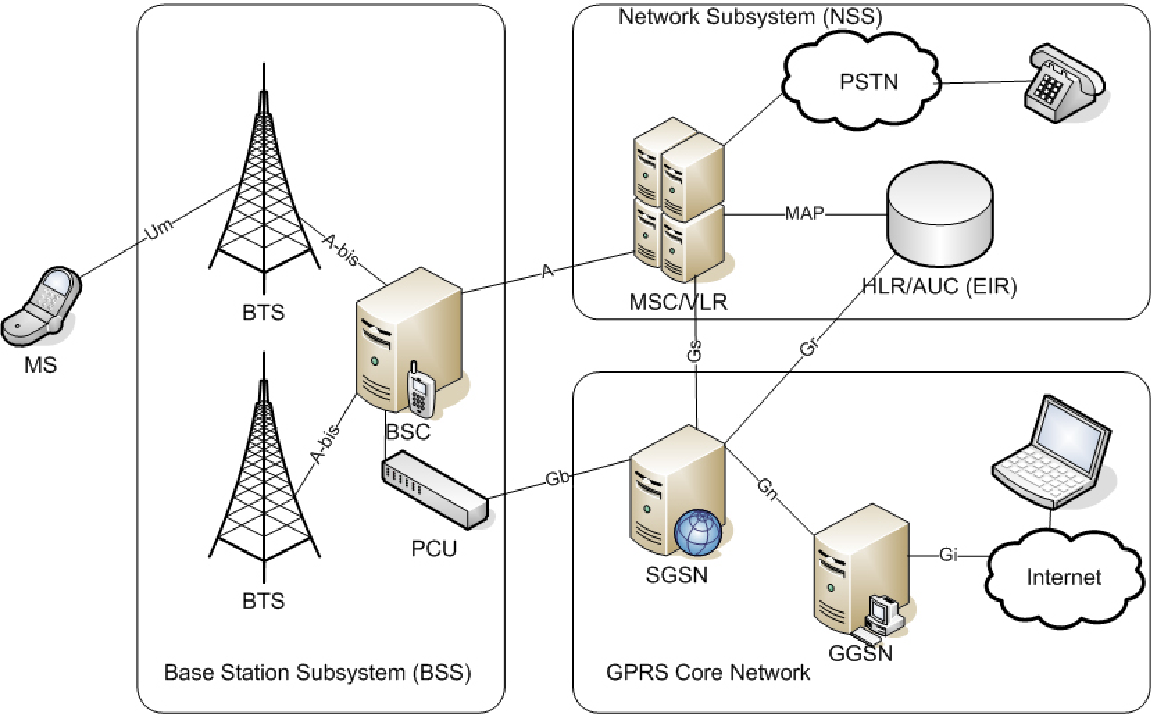
\includegraphics[width=0.7\textwidth]{images/3g-umts.png}
    \caption{Architettura UMTS}
\end{figure}


\subsection{HSPA/HSPA+}
Evoluzione del UMTS per consentire velocità maggiori apportando modifiche nella trasmissione del segnale.
Con questo nuovo standard si riescono a raggiungere velocità di 42 Mb/s\cite{hspa}.

\clearpage

\section{4G}
La quarta generazione è al momento quella più utilizzata, permette di avere dei servizi basati su velocità molto alte. 
A differenza delle precedenti generazioni che dovevano gestire due \textit{core network}: uno per la rete telefonica e un altro
per \textit{internet}, per la prima volta il 4G introduce un unico \textit{core network} basato su \textit{Internet Protocol} (IP).\\
Per consentire un aumento consistente della velocità le maggiori modifiche di questa generazione sono state apportate nella \textit{radio interface}, mentre
l'architettura rimane con una struttura simile a quella precedente.
\subsection{LTE}
Il \textit{Long Term Evolution} è uno standard di quarta generazione che ha i seguenti componenti architetturali\cite{lte}:
\begin{itemize}
    \item \textit{Home Subscriber Server} (HSS) è il \textit{database} centrale dei \textit{subscriber} come l'HLR del GSM/UMTS.
    \item \textit{Mobility Management Entity} (MME) il corrispettivo del VLR in GSM/UMTS.
    \item \textit{Serving - Gateway} (S-GW) è un componente che svolge il ruolo di \textit{router} indirizzando i dati dalla \textit{base station}
    al P-GW.
    \item \textit{Packet data network - Gateway} (P-GW) è il componente per interfacciare il \textit{core network} con \textit{internet}.
    \item \textit{Policy Control and Charging Rules Function} (PCRF) è un componente responsabile delle regole di gestione per il flusso di informazioni.
\end{itemize}
\begin{figure}[ht]
    \centering
    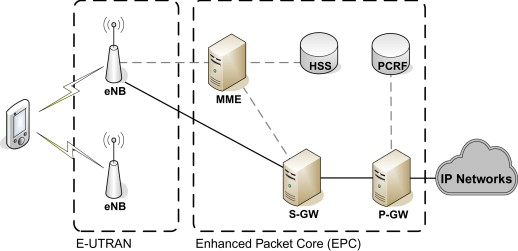
\includegraphics[width=0.8\textwidth]{images/4g-lte.jpg}
    \caption{Architettura LTE}
\end{figure}

\clearpage

\section{5G}
Il 5G, ovvero lo standard di quinta generazione rappresenta l'ultima frontiera della tecnologia cellulare.
Il suo principale scopo è consentire l'\textit{Internet of Things} massivo, ossia un \textit{network} che sia 
in grado di gestire la connessione di molti dispositivi con latenze molto piccole.
Per consentire velocità fino a 10 Gb/s si sono
dovute apportare importanti modifiche strutturali che rendono la sua architettura molto diversa da quelle viste fin'ora.\\
L'architettura implementata prende il nome di \textit{Service-Base Architecture} (BSA).
La BSA consiste nel dividere tutte le funzioni in una serie di \textit{microservices}\cite{5g-approach}. 
Questa nuova struttura è stata introdotta per garantire la scalabilità del sistema, migliorare le prestazioni (velocità) e per 
permettere di realizzare il \textit{massive IOT}, che richiede la gestione simultanea di molti dispositivi.\\
I principali blocchi che la compongono sono:
\begin{itemize}
    \item AMF \textit{Core Access and Mobility Management Function} responsabile dell'autenticazione e localizzazione del dispositivo.
    \item SMF \textit{Sesson Management Function} per la gestione della sessione di ogni UE.
    \item PCF\textit{Policy Control Function} per la gestione delle \textit{policy}.
    \item UDM \textit{Unified Data Management} per la gestione dell'identità dell'utente, questo compito era precedentemente svolto da HSS o HLR.
    \item AUSF \textit{Authentication Server Function} per effettuare l'autenticazione dell'utente.
    \item SDSF \textit{Structured Data Storage Network Function} è un helper per la memorizzazione di dati strutturati.
    \item UDSF \textit{Unstructured Data Storage Network Function} è un helper per la memorizzazione di dati non strutturati.
    \item NEF \textit{Network Exposure Function} per esporre determinate funzionalità a servizi di terze parti.
    \item NRF \textit{NF Repository Function} per scoprire tutti i servizi disponibili.
    \item NSSF \textit{Network Slicing Selector Function} per selezionare una determinata partizione di \textit{network}.
    \item UPF \textit{User Plane Function} trasporta il traffico dal RAN all'internet.
\end{itemize}
\begin{figure}[ht]
    \centering
    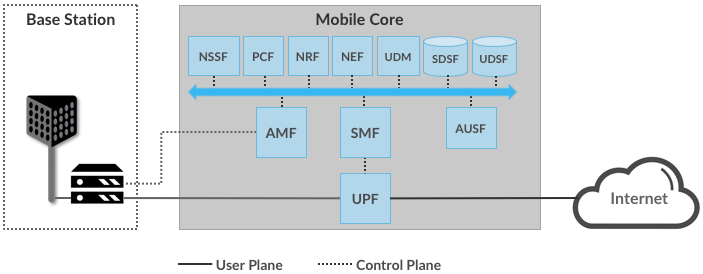
\includegraphics[width=0.8\textwidth]{images/5g-planes.png}
    \caption{Architettura 5G\cite{5g-approach}}
\end{figure}

\clearpage

\subsection{Network Slicing}
Il \textit{Network Slicing} rappresenta una delle caratteristiche più importanti del 5G. Con questo termine si intende il partizionamento della
rete in diversi "piani" ciascuno con caratteristiche e requisiti particolari, indipendente e autonomo. Questo risulta fondamentale nella realizzazione 
dell' IOT massivo, infatti in questo modo la gestione del traffico terrà conto dell'applicazione che viene utilizzata nel dispositivo per decidere quali prestazioni sono 
richieste da quel dispositivo.
\begin{figure}[ht]
    \centering
    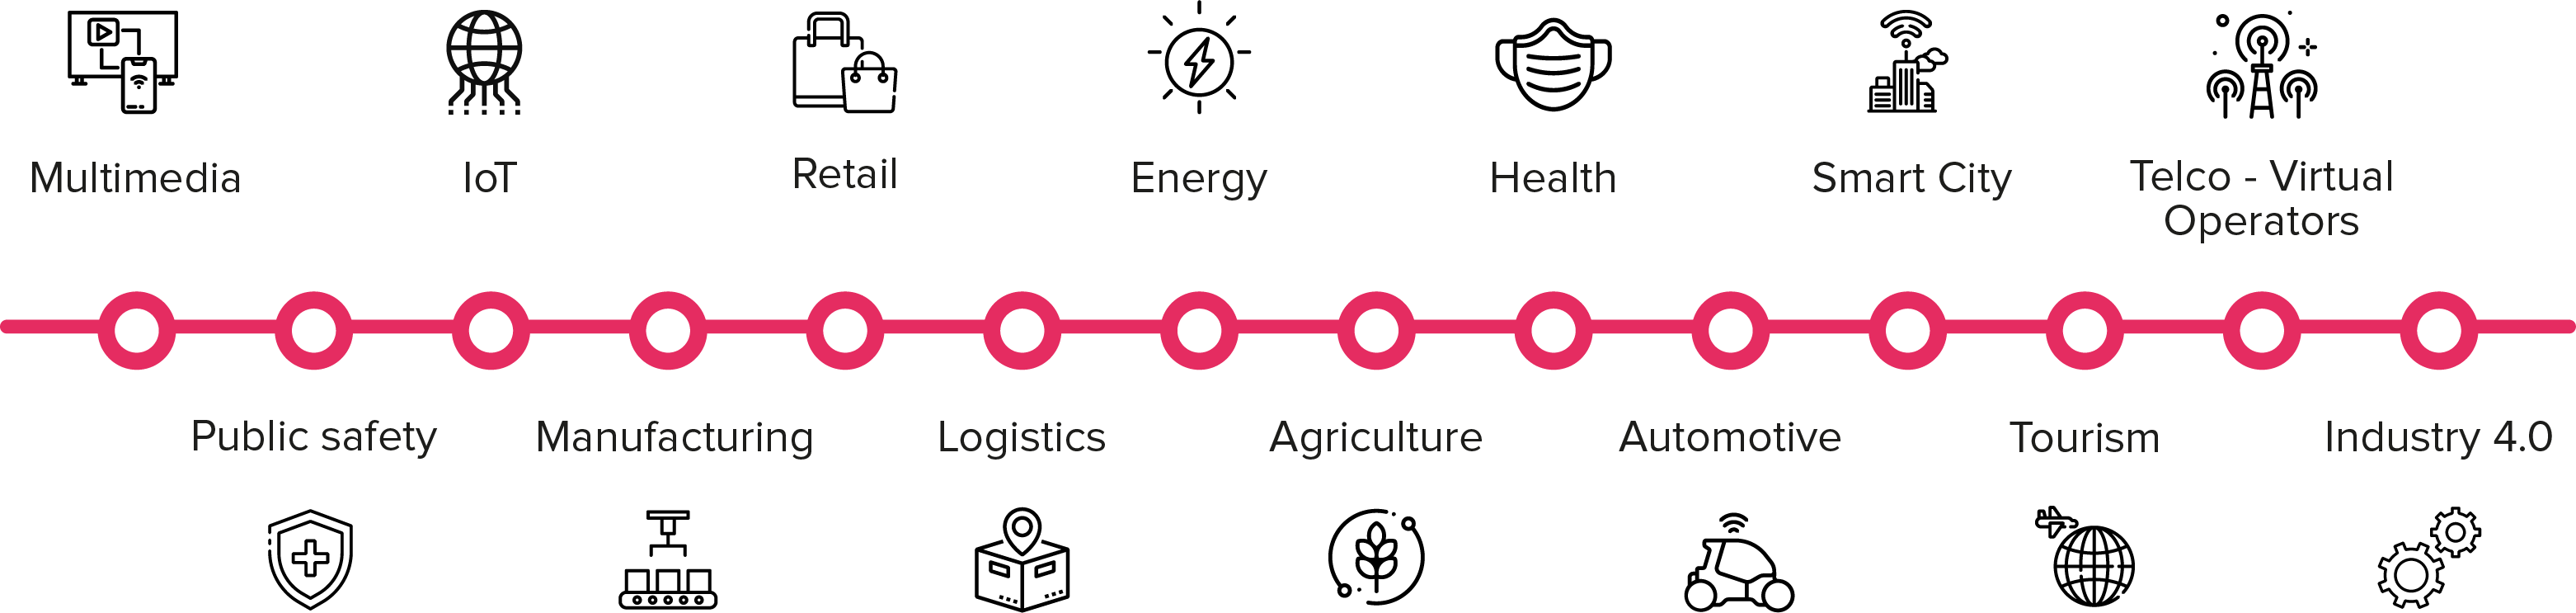
\includegraphics[width=0.8\textwidth]{images/5g-eg-of-use.png}
    \caption{Esempi di applicazioni per il 5G}
\end{figure}\\
Ogni segmento virtuale del network ha uno specifico identiicativo che deve essere indicato nella fase di autenticazione come verrà illustrato nella sezione 5.3. Per ogni \textit{slice} sono 
richieste delle prestazioni differenti, per esempio il settore delle \textit{critical communication} deve avere delle latenze molto basse.
\begin{figure}[ht]
    \centering
    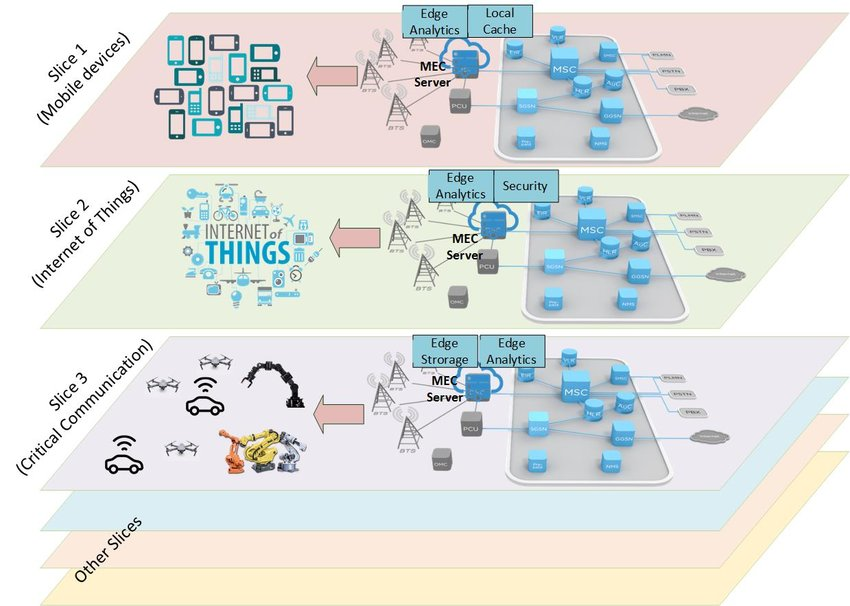
\includegraphics[width=0.8\textwidth]{images/5g-slicing.jpg}
    \caption{\textit{Network slicing} nel 5G}
\end{figure}\\
La realizzazione del \textit{Network Slicing} avviene tramite i \textit{Software Degined Network} che nella prossima sezione verranno approfonditi.

\clearpage

\subsection{\textit{Software Defined Network} e  \textit{Network Function Virtualization}}
I \textit{Software Defined Network} (SDN) sono dei programmi per la virtualizzazione della rete. Sono necessari per interfacciarsi a livello applicativo con i dispositivi cellulari 
in modo da gestire il traffico della rete in modo efficace\cite{5g-sdn}.
    \clearpage
    \chapter{Attacco Denial of Service}
L'attacco di tipo \gls{dos} consiste nel rendere non disponibili servizi offerti da computer o altri
dispositivi \cite{dos-definition}. Questo avviene esasperando di richieste la macchina o infrastruttura che viene scelta come
vittima.

\section{Vulnerabilità nelle reti cellulari}
Le reti cellulari non sono esenti da questo tipo di attacchi, anzi, sono uno degli obiettivi più ambiti e sopratutto difficile da risolvere
poichè le vulnerabilità che sfruttano sono spesso organiche nell'architettura della rete.
Sono diversi i componenti che possono essere vulnerabili a un attacco DOS in una rete cellulare, gli obiettivi identificati come ottimi sono quelli
che comportano un maggior utilizzo delle risorse della rete.\\
Nelle prossime sezioni verranno illustrate le principali metodologie per fare un attacco di tipo \gls{dos} alle reti cellulari\cite{4g-dos-recap}.

\clearpage

\subsection{Radio Jamming}
Il \textit{Radio Jamming} è una tipologia di attacco \textit{Denial of Service} che consiste nel disturbare il segnale cellulare emettendo delle onde radio.
La realizzazione di questo tipo di attacco è molto semplice, basta procurarsi un trasmettitore che invia segnali ad alta energia nella banda cellulare di riferimento.\\
Un miglioramento del classico \textit{radio jamming} è lo \textit{smart jamming} che consiste nel saturare uno o più canali di comunicazione della rete. Questo fa sembrare 
il \textit{network} non disponibile a tutti gli utenti collegati a quella determinata cella.
\begin{figure}[h]
    \centering
    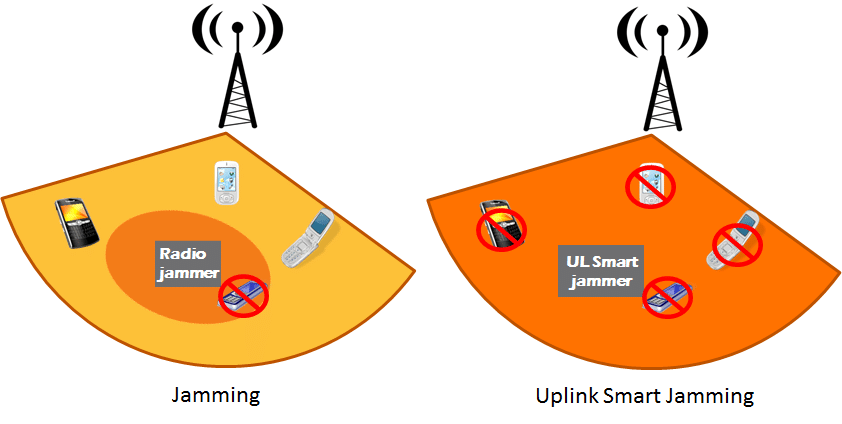
\includegraphics[width=0.6\textwidth]{images/dos-jamming.png}
    \caption{\textit{radio} e \textit{smart jamming}\cite{4g-dos-recap}}
\end{figure}\\

\subsection{Vulnerabilità di sistema}
Un altro classico modo per creare un interruzione di sistema in una rete cellulare è sfruttando le classiche vulnerabilità che si presentano spesso in qualsiasi tipo di computer.
Questo ovviamente perchè tutta l'architettura di una rete cellulare non è altro che \textit{server} con specifiche particolari.

\subsection{Botnet}
Questa è sicuramente una delle tipologie più diffuse, ed è modo con cui si realizzano i \gls{ddos}. L'attaccante, in questo caso, dispone del controllo di 
un grande numero di dispositivi infettati da \textit{malware} che possono essere attivati da lui per esasperare di richieste un determinato servizio.
\begin{figure}[h]
    \centering
    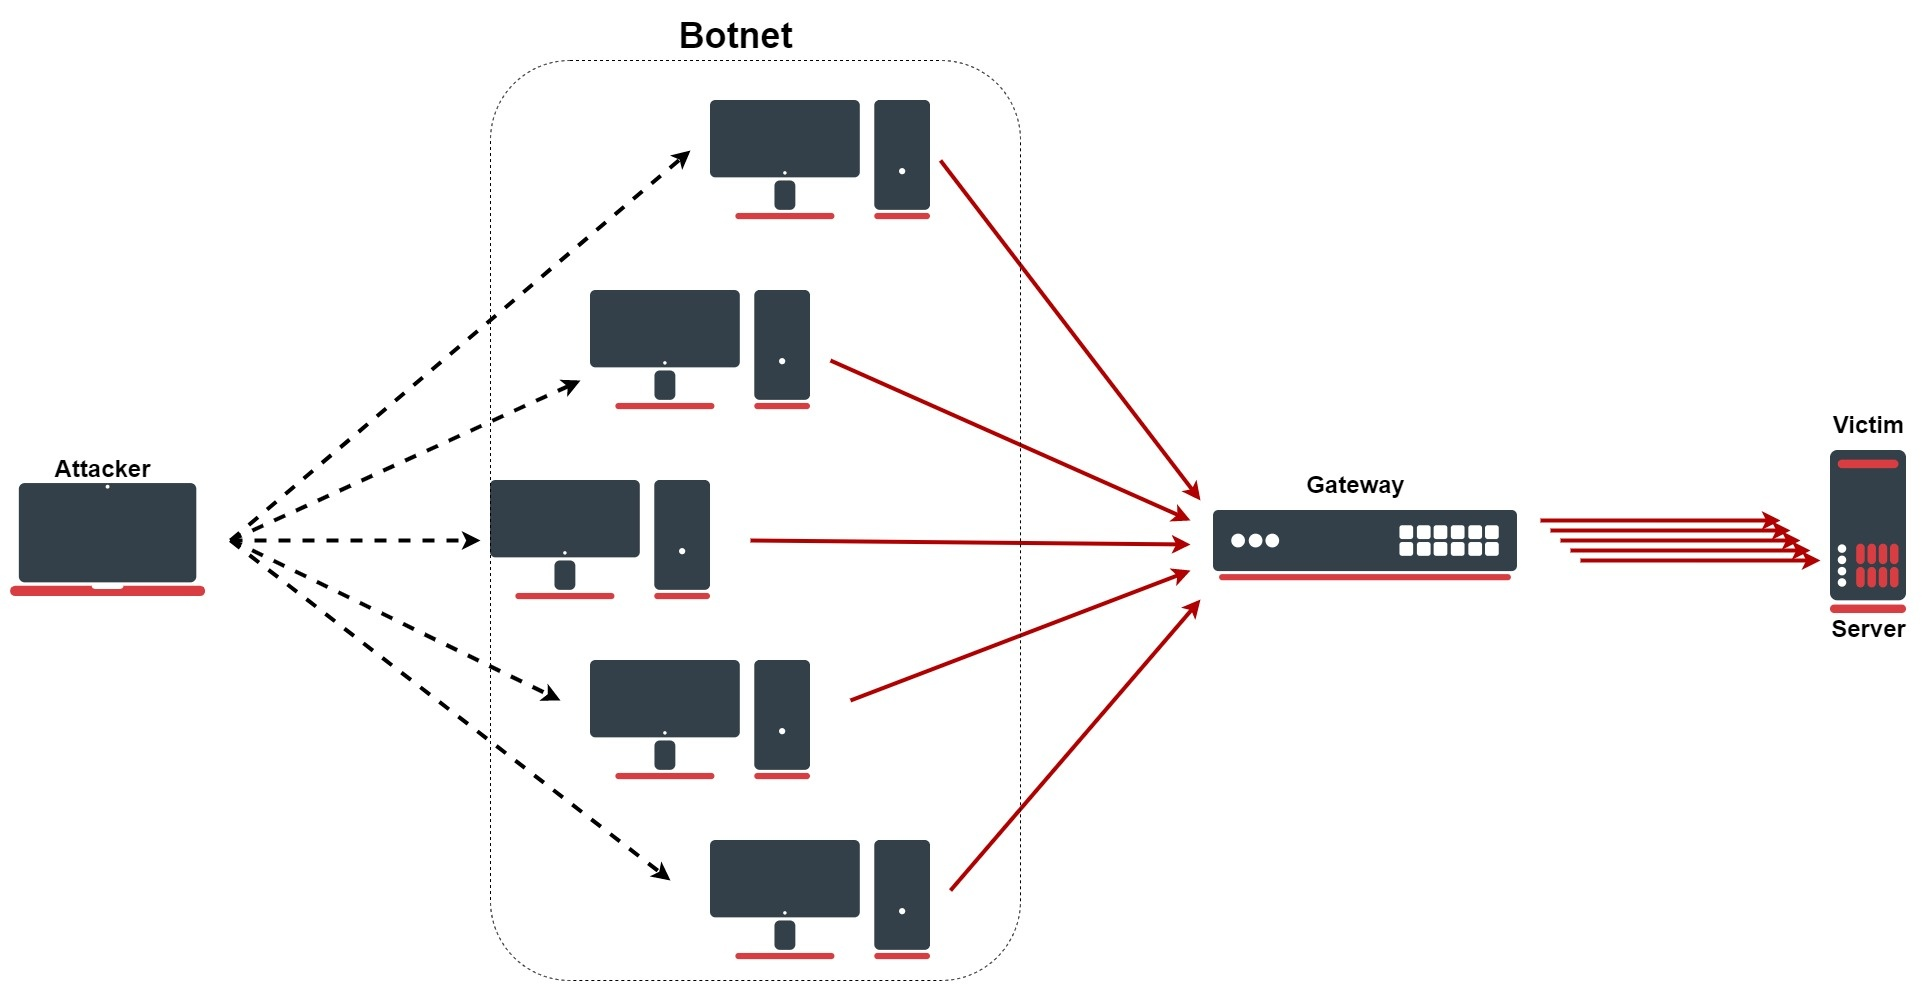
\includegraphics[width=0.5\textwidth]{images/ddos.jpg}
    \caption{\textit{Distributed Denial of Service}}
\end{figure}\\

\subsection{Autenticazione}
Questo è uno degli attacchi più pericolosi poichè le vulnerabilità che sfrutta sono molto difficile da risolvere dato che sono intrinseche nell'architettura del sistema.
È la tipologia di vulnerabilità che è stata scelta per confrontare la sicurezza dell'architettura 5G con quelle precedenti.
Il suo funzionamento si basa sull'esasperare di richieste di autenticazione i sistemi identificativi delle reti cellulari, che solitamente 
sono i componenti con più traffico della rete come la HLR nelle reti 2G/3G.\\
Questa vulnerabilità si trova nel meccanismo di autenticazione dei dispositivi denominato \gls{aka} dove un dispositivo
non autenticato forza delle computazioni all'interno del \textit{core network} che consumano più risorse della richiesta stessa\cite{umts-dos}.
Ad aumentare la pericolosità di questa vulnerabilità è la possibilità di creare computazioni nel \textit{core network} senza essere effettivamente autenticati, e quindi 
senza disporre di una \gls{sim} valida. Questa tipologia di attacchi, definiti come SIM-less, verranno presi come riferimento per sfruttare questa vulnerabilità come illustrato per le 
reti \gls{gsm}\cite{gsm-dos-simless} e \gls{umts}\cite{umts-dos}.



\section{Misurazione}
Per capire quale componente della rete sia il più vulnerabile a un attacco \gls{dos} si devono fare delle misurazioni sui vari componenti del \textit{network}.
In questo modo è possibile capire in quale punto si possono creare dei rallentamenti o \textit{bottleneck} dovuti a un sovraffollamento di richieste.\\
In \cite{measuring-dos} vi è una dettagliata spiegazione di come procedere con queste misurazioni e sopratutto come quantificare il numero di dispositivi che 
servono all'attaccante per completare l'attacco con successo.\\
Solitamente le statistiche riguardo alle prestazioni dei componenti del \textit{network} non sono direttamente fornite dagli operatori telefonici quindi bisogna 
basarsi sui tempi di risposta. Per esempio, l'immagine seguente mostra i tempi di risposta della \gls{hlr} in una rete \gls{umts} al comando \textit{location updates}.
\begin{figure}[h]
    \centering
    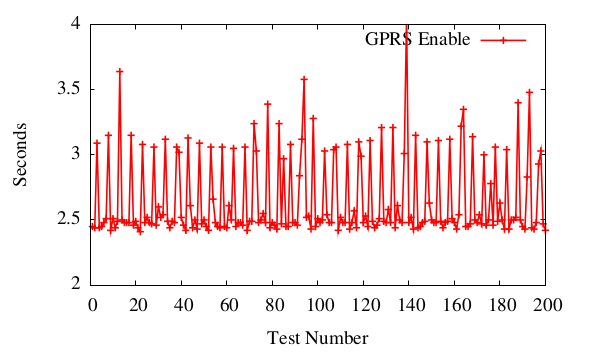
\includegraphics[width=0.7\textwidth]{images/hlr-measuring.png}
    \caption{Misurazione tempi di risposta \gls{hlr} con \textit{location updates}\cite{measuring-dos}}
\end{figure}
    \clearpage
    \chapter{Sistema di autenticazione}
Il meccanismo di autenticazione è la procedura per verificare che un determinato dispositivo
sia abilitato a connettersi alla rete.
Questo procedimento avviene tramite l'\textit{Authentication and key agreement} (AKA), procedimento in cui
il \textit{core network} abilita un dispositivo a connettersi, e come vedremo, dal 3G anche viceversa (autenticazione mutua).\\
In questo capitolo verranno trattati le procedure di autenticazione\cite{identifications} per le generazioni dal 2G al 5G, il 1G è stato escluso 
poiché ha un funzionamento completamente analogico.

\clearpage

\section{2G}
Il sistema di autenticazione di seconda generazione utilizza principalmente due codici univoci della SIM e del MS:
\begin{itemize}
    \item \textit{International Mobile Subscriber Identity} (IMSI) ovvero un codice identificatvo della SIM
    \item \textit{International Mobile Equipment Identity} (IMEI) ovvero un codice identificativo del MS
\end{itemize}
Questi due codici saranno necessari anche per le prossime generazioni fino al 4G.\\
La procedura di autenticazione di un MS segue questi passaggi:
\begin{enumerate}
    \item Il MS invia l'IMSI alla BTS di riferimento che lo inoltra al \textit{core network}, questo
    avviene ogni volta che il MS vuole connettersi al \textit{network} e non risulta già registrato presso 
    la rete di riferimento. In caso lo fosse, verrà utilizzato il TMSI \textit{Temporary MobileSubscriber Identity}
    per preservare il suo anonimato.
    \item L'AuC cerca la chiave Ki associata all'IMSI e insieme a un numero casuale RAND genera un codice SRES che verrà
    salvato nel VLR.
    \item Viene inviato al MS il RAND generato.
    \item La stessa procedura viene fatta dal MS, che genera quindi il suo SRES e lo invia al VLR.
    \item Il VLR confronta se l'SRES ricevuto corrisponde a quello generato dall'AuC, se corrispondono l'autenticazione risulta
    effettuata con successo.
\end{enumerate}

\begin{figure}[h]
    \centering
    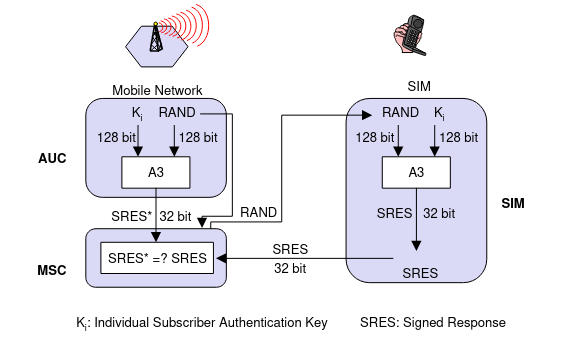
\includegraphics[width=0.7\textwidth]{images/auth-2g.png}
    \caption{Autenticazione nelle reti 2G}
\end{figure}

\clearpage

\section{3G-4G}
Dato che l'autenticazione nelle reti 3G e 4G è molto simile, verranno trattate insieme in questa sezione.
L'autenticazione nell'architettura di terza e quarta generazione è molto simile a quella della seconda salvo i seguenti miglioramenti:
\begin{itemize}
    \item Viene introdotta l'autenticazione mutua per prevenire l'autenticazione a false \textit{base stations}.
    \item La lunghezza della chiave Ki viene incrementata da 64 a 128 bit.
    \item Viene implementato un flag per verificare se le comunicazioni vengono compromesse durante la trasmissione chiamato \textit{Integrity Key} (IK).
\end{itemize}
Il procedimento di autenticazione è il seguente\cite{4g-auth}:
\begin{enumerate}
    \item Il MS invia l'IMSI alla BTS di riferimento che lo inoltra al \textit{core network}.
    \item L'AuC cerca la chiave Ki associata all'IMSI e insieme a un numero casuale RAND genera un codice SRES che verrà
    salvato nel VLR.
    \item Viene trovata la chiave Ki corrispondente all'IMSI dall'AuC, dopodichè viene generato un codice SRES con l'utilizzo di un numero randomico RAND.
    Inoltre, viene generato un codice AUTN per permettere al MS di autenticare il \textit{network}.
    \item Viene inviato al MS il RAND e AUTN.
    \item Il MS autentica il \textit{network} confrontando il valore di AUTN ricevuto. Se il \textit{network} è valido, prosegue con la generazione del SRES.
    \item Il VLR confronta se il SRES ricevuto corrisponde a quello generato dall'AuC, se corrispondono l'autenticazione risulta
    effettuata con successo e viene generato,salvato e inviato il TMSI.
\end{enumerate}
\begin{figure}[h]
    \centering
    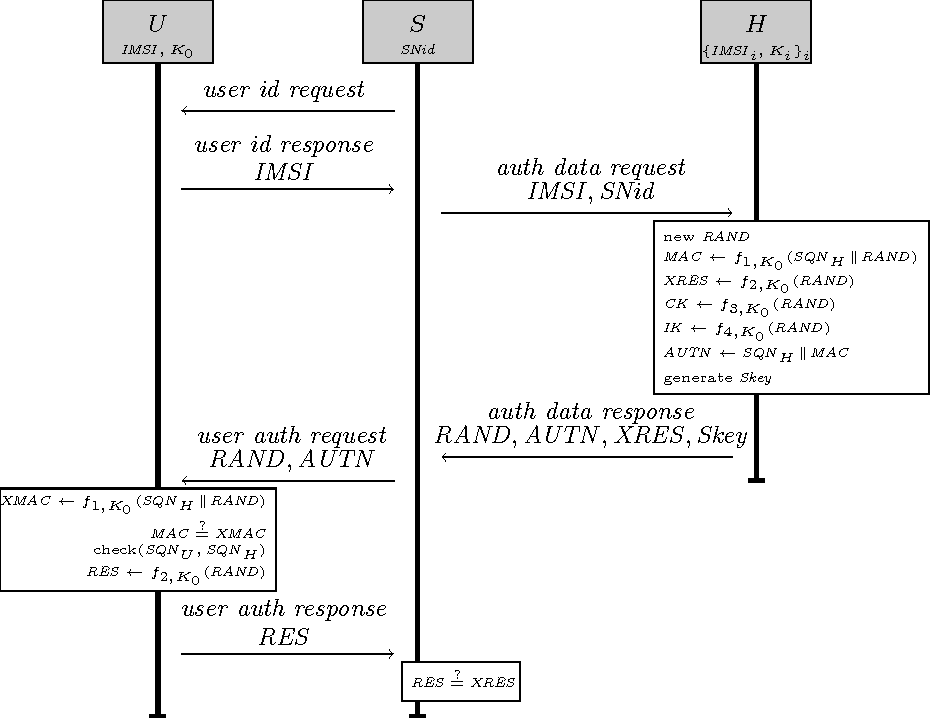
\includegraphics[width=0.7\textwidth]{images/auth-3g.png}
    \caption{Autenticazione nelle reti 3G-4G}
\end{figure}

\clearpage

\section{5G}
L'autenticazione della generazione 5G è molto diversa dalle precedenti poichè, come illustrato nella sezione 3.5, l'architettura è completamente rivista diventando una ramificazione di microservizi.
Sono definiti tre protocolli di autenticazione:
\begin{itemize}
    \item 5G-AKA: 5G-Authentication and Key Management
    \item EAP-AKA: Extensible Authentication Protocol – Authentication and Key Management
    \item EAP-TLS: Extensible Authentication Protocol – Transport Layer Security
\end{itemize}
Rispetto alle generazioni precedenti ci sono stati i seguenti miglioramenti di sicurezza\cite{5g-vs-4g}:
\begin{itemize}
    \item L'IMSI non viene mai comunicato in chiaro ma sempre criptato
    \item I componenti del \textit{network} coinvolti sono dei servizi
\end{itemize}
L'autenticazione è fondamentalmente diviso in due parti: La prima è l'inizializzazione dell'autenticazione e la scelta del metodo di autenticazione.
La seconda è invece l'autenticazione mutua come avviene nelle generazioni precedenti.
Lo schema di autenticazione è il seguente\cite{5g-auth}:
\begin{enumerate}
    \item Il MS invia il SUCI o 5G-GUTI alla BTS di riferimento che lo inoltra al AMF/SEAF,
    il GUTI è un identificativo temporaneo simile al TMSI delle generazioni precedenti, invece il SUCI è un identificatore criptato
    permanente.
    \item il SEAF manda l'identificatore del dispositivo (SUCI o 5G-GUTI) e il \textit{Serving Network Name} (SNN) all'AUSF.
    Il SNN è una concatenazione di codici identificativi di servizi e il codice identificativo del \textit{Serving Network}. Serve per capire 
    a quale \textit{slice} vuole connettersi il dispositivo.
    \item L'AUSF controlla che la richiesta dal SEAF sia autorizzata a utilizzare il SNN, in caso non lo fosse risponde con un 
    apposito messaggio di errore.
    \item L'AUSF reperisce la chiave associata all'identificativo nell'archivio UDM e genera il rispettivo SRES con un numero randomico RAND.
    \item Viene inviato all'MS il RAND e AUTN (per l'autenticazione mutua).
    \item Il MS procede con la creazione del SRES e lo invia al SEAF.
    \item Il SEAF inoltra il SERS all'AUSF che si occupa di controllare se corrispondono e in caso confermare l'autenticazione.
\end{enumerate}
\begin{figure}[h]
    \centering
    \includegraphics[width=0.8\textwidth]{images/auth-5g.png}
    \caption{Autenticazione nelle reti 5G}
\end{figure}
    \clearpage
    \section{Attacco alle reti UMTS}
\subsection{Funzionamento}
\subsection{Analisi dei risultati}
    \clearpage
    \chapter{Attacco all'autenticazione delle reti 5G}
In questa sezione verranno trattate le vulnerabilità riguardo un attacco di tipo \gls{dos} all'autenticazione delle reti 5G.
Questa generazione ha risolto alcune delle probematiche legate all'autenticazione, come per esempio a differenza del 4G \gls{lte} l'identificatore 
del \gls{ms} viene criptato con la chiave pubblica prima di essere inviato al \textit{core network}, evitando così di poter essere intercettato e rubato\cite{5g-vs-4g}.
Però, con il grande aumento di dispositivi connessi che questa tecnologia vuole incentivare, per esempio nel mondo dell' \gls{iot}, gli attacchi \gls{dos} saranno senz'altro più 
semplici da realizzare.\\
I \gls{sdn} e \gls{nfv}, componenti fondamentali per garantire le eccezionali prestazioni del 5G, potrebbero essere un efficace strumento di monitoraggio per identificare possibili 
attacchi come spiegato in \cite{dos-detection-with-sdn}.\\
Allo stesso tempo però, la centralizzazione del controllo del \textit{network} con un \gls{sdn} e \gls{nfv} crea le condizioni ottimali per effettuare un attacco \gls{dos} con successo\cite{5g-dos}.\\
Questa tipologia di attacchi che ha lo scopo di creare una interruzione del servizio hanno una pericolosià maggiore in questa generazione. Infatti, il mondo dell'\gls{iot} e le smart cities comprendono 
dispositivi sensibili come per esempio il mondo della telemedicina.

\clearpage

\section{IMSI \textit{catching}}
Come anticipato, l'avanzamento più importante in termini di sicurezza che questa nuova generazione ha apportato è sicuramente la trasmissione dell'identificativo del \gls{ms} in forma 
criptata. Questa innovazione ha reso molto più difficile la pratica dell'\gls{imsi} \textit{catching} trattata nella sezione 6.2 fondamentale per effettuare un attacco \gls{dos}.\\
Realisticamente però bisogna sottolineare che questa pratica non risulta completamente debellata. Infatti, tutte le nuove reti 5G, come è stato anche per le generazioni precedenti, devono 
essere retro compatibili, e quindi per un non determinato lasso di tempo devono essere supportate le procedure degli \textit{standard} precedenti che, come spiegato nel capitolo precedente, soffrono 
di questa vulnerabilità.\\
In \cite{suci-catch} viene illustrato un metodo per effettuare un attacco \gls{mitm} nelle reti 5G in modo da ottenere l'\gls{imsi} criptato dell'utente: il \gls{suci}. Questo metodo però non sarebbe applicabile per effettuare 
una raccolta di identificativi per poi effettuare un attacco \gls{dos} poichè il \gls{suci} viene rigenerato dopo ogni utilizzo.
\begin{figure}[ht]
    \centering
    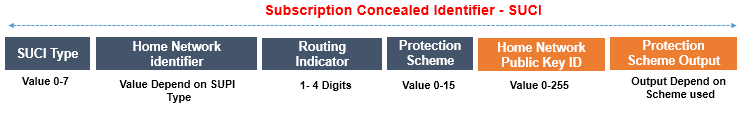
\includegraphics[width=0.8\textwidth]{images/5g-suci.png}
    \caption{Composizione del SUCI nel 5G}
\end{figure}

\section{Replicazione dell'attacco SIM-less}
Alla base degli attacchi trattati nella sezione 6.3 vi è la costruzione di un \textit{database} di \gls{imsi}. Questo \textit{database} può essere agevolmente costruito nelle generazioni precedenti al 5G 
tramite le tecniche di \gls{imsi} \textit{catching} trattate in 6.2. Nel 5G risulta molto più difficile creare un archivio di IMSI poichè questi viaggiano in forma criptata nella rete, ovvero comunicando il \gls{suci}.\\
Tuttavia, se si riuscisse a ottenere comunque un \textit{database} di \gls{imsi} rubati si potrebbe ottenere un attacco dello stesso tipo di \cite{gsm-dos-simless} e \cite{umts-dos} con prestazioni migliori 
perchè il nuovo protocollo 5G NR\cite{5g-nr} per l'\textit{air interface} è stato progettato per supportare il \textit{Massive Machine Type Communications} ovvero l'\gls{iot} massivo che richiede latenze molto basse e capacità molto alte.
Per questo, sicuramente la capacità dei canali di comunicazione durante la procedura di autenticazione avrebero un valore di TPS molto alto, sufficiente a causare un notevole degradamento delle prestazioni.

\section{Nuove vulnerabilità}
L'implementazione del \gls{suci} e \gls{supi} ha risolto, o quantomeno reso molto più complicata la pratica dell'\gls{imsi} \textit{catching}. Allo stesso tempo però ha incrementato il dispendio di risorse durante l'autenticazione
di un dispositivo. Come è chiaramente visibile nell'immagine sottostante, prima della generazione dei vettori di autenticazione vengono innestate delle procedure per decriptare il \gls{suci} che avvengono con un algoritmo detto 
\gls{ecies}. 
Questa procedura aumenta inevitabilmente la creazione di possibili DOS all'autentcazione. 
In \cite{5g-lightweight} è descritto un protocollo che permetterebbe di controllare fin dal primo momento se il \gls{ms} ha un \gls{suci} valido senza incorrere nella decriptazione.

    \clearpage
    \chapter{Conclusioni}
    \clearpage
    \printbibliography
\end{document}